%!TEX root = ../report.tex

\begin{document}
    \chapter{Theoretical Background}
    In this chapter the we will introduce the reader with the theoretical primers needed to comprehend this work in depth. 

    \section{Camera Geometry}
    A camera in simple words is mapping or projecting of 3d world points on an image plane. To understand how this mapping works we need to understand first the camera model which is defined using the tools of geometry. In computer there are two typed of camera models finite and infinite, which are divided on the basis of the distance of camera from the 3D real world points. In finite camera model the camera center lies at the finite distance distance from the 3D world point where this is vice versa in infinite camera model. In our case we will consider the finite camera model as it forms the basis of camera systems we use in the real world. 
    
    Generally the camera mapping or projection of 3d world point on the image plane is represented by camera matrix which is of size $3x4$, this matrix has 11 degrees of freedom. This matrix is can be divided into intrinsic and extrinsic camera matrix. To derive this camera mapping first we need to understand what is pin hole camera geometry. 
    
     \begin{figure}[h]
    \centering
    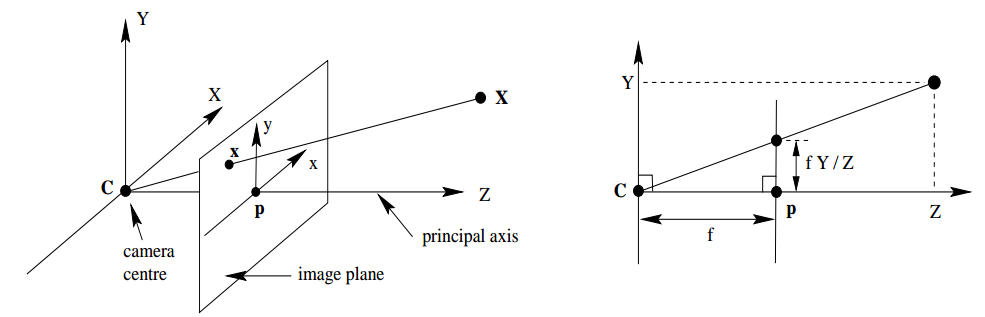
\includegraphics[width=\textwidth]{images/pinhole_camera.png}
    \caption{Pinhole camera geometry \cite{10.5555/861369}}
    \end{figure}
    
    Considering the central projection of 3D point \txtbf{X} on to the image plane. Let the camera center is at the center of origin of euclidean space. The image plane is at distance $z = f$. Pinhole camera model maps the point  \textbf{X} $ = (X, Y, Z)^{T}$ to the image plane, where a line from point \textbf{X} intersects the image plane at point \textbf{x} and meets the center of projection. This center of projection is also called camera center or optical center. Thus, using the similar triangles we can compute the mapping of $ (X, Y, Z)^{T}$ to $(fX/Z, fY/Z, f)^{T}$ which lies on the image plane. Therefore this projection can be seen as the mapping from $IR^{3}$ to $IR^{2}$ in euclidean space. 
    
    Assuming the world and image points to be homogeneous vectors this mapping can be represented as:
   \begin{center}
$\left(\begin{array}{c}X \\ Y \\ Z \\ 1 \end{array}\right) \rightarrow \left(\begin{array}{c} fX \\ fY \\ Z \end{array}\right) = \begin{bmatrix}f & & & 0 \\  &f & & 0  \\   & &1 & 0   \end{bmatrix}\left(\begin{array}{c}X\\ Y  \\Z \\ 1 \end{array}\right)$

\end{center}
    
The above equation can be represented as  $X^{‘} = PX $. Where X is the real world point represented in the homogenous coordinates as $(X, Y, Z, 1)^{T}$ and P is a $3x4$ homogeneous matrix called camera projection matrix. P in this case can be rewritten as $diag(f,f,1) [I|0]$, where diag(f,f,1) is a $3x3$ matrix and $[I|0]$ is a zero column vector. 
Generally the origin of coordinated is not at the optical center, there exists some offset. So the mapping in that case will change: 
\begin{center}
$(X,Y,Z)^{T} \rightarrow (fX/Z + p_{x}, fY/Z + p_{y})^{T}$
\end{center}
 where $(p_{x}, p_{y})^{T}$ are the coordinates of the new optical center. So according to this mapping can be expressed as:
   \begin{center}
$\left(\begin{array}{c}X \\ Y \\ Z \\ 1 \end{array}\right) \rightarrow \left(\begin{array}{c} fX + Zp_{x} \\ fY + Zp_{y} \\ Z \end{array}\right) = \begin{bmatrix}f & &p_{x} & 0 \\  &f &p_{y} & 0  \\   & &1 & 0   \end{bmatrix}\left(\begin{array}{c}X\\ Y  \\Z \\ 1 \end{array}\right)$

And $ K =  \begin{bmatrix}f & &p_{x} \\  &f &p_{y}  \\   & &1    \end{bmatrix}$
\end{center}
 Here K is called camera calibration matrix. The 3D world point is generally in the world coordinate frame and in most of the cases there exists some rotation and translation between the camera coordinate frame and world coordinate frame.
 
    \begin{figure}[h]
    \centering
    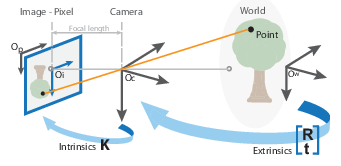
\includegraphics[width=8cm, height =4cm]{images/camera_geo.png}
    \caption{ Real world coordinates are transformed to camera coordinate frame using extrinsic matrix \cite{10.5555/861369}}
    \end{figure}
    
    This rotation and translation is generally represented as 3x4 matrix, $[R | C ]$ called extrinsic matrix, where $R$ is the rotation matrix and $C$ is the translation matrix. The above derived mapping assumes that the image plane is of similar scale in x and y direction, but in most of the cases it is not true. To counter this problem with the assumption that image coordinates are represented in the form of pixels we will introduce a scale factor here in x and y direction as $m_{x}$ and $m_{y}$ and we further introduce on more factor called skew coefficient $s$ in the cases when x and y axis of camera frames are not perpendicular to each other. Thus the resulting camera matrix can be represented as:
        \begin{center}
$K =  \begin{bmatrix} \alpha_{x} & s &c_{x} \\  0 & \alpha_{y} & c_{y}  \\  0  &0 &1 \end{bmatrix}$
    \end{center}
    
    So we can summarize this mapping from real world to camera plane, first the real world coordinates are transferred to camera coordinate frame via extrinsic matrix and the resulting points in camera coordinate frames are projected to image plane using camera matrix or camera calibration matrix. 
        \begin{figure}[h]
    \centering
    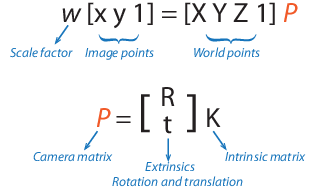
\includegraphics[width=8cm, height =4cm]{images/extrinsic_intrinsic.png}
    \caption{ Projection of a real world point onto image plane using camera geometry \cite{10.5555/861369}}
    \end{figure}
    
   
   
    \section{Inverse Perspective Transform}
    
    \section{Hough Transform}
    
    \section{A Brief Guide to Convolutional Neural Networks}
    
    \section{Semantic Segmentation}
    
\end{document}
